% Options for packages loaded elsewhere
\PassOptionsToPackage{unicode}{hyperref}
\PassOptionsToPackage{hyphens}{url}
%
\documentclass[
]{book}
\usepackage{lmodern}
\usepackage{amssymb,amsmath}
\usepackage{ifxetex,ifluatex}
\ifnum 0\ifxetex 1\fi\ifluatex 1\fi=0 % if pdftex
  \usepackage[T1]{fontenc}
  \usepackage[utf8]{inputenc}
  \usepackage{textcomp} % provide euro and other symbols
\else % if luatex or xetex
  \usepackage{unicode-math}
  \defaultfontfeatures{Scale=MatchLowercase}
  \defaultfontfeatures[\rmfamily]{Ligatures=TeX,Scale=1}
\fi
% Use upquote if available, for straight quotes in verbatim environments
\IfFileExists{upquote.sty}{\usepackage{upquote}}{}
\IfFileExists{microtype.sty}{% use microtype if available
  \usepackage[]{microtype}
  \UseMicrotypeSet[protrusion]{basicmath} % disable protrusion for tt fonts
}{}
\makeatletter
\@ifundefined{KOMAClassName}{% if non-KOMA class
  \IfFileExists{parskip.sty}{%
    \usepackage{parskip}
  }{% else
    \setlength{\parindent}{0pt}
    \setlength{\parskip}{6pt plus 2pt minus 1pt}}
}{% if KOMA class
  \KOMAoptions{parskip=half}}
\makeatother
\usepackage{xcolor}
\IfFileExists{xurl.sty}{\usepackage{xurl}}{} % add URL line breaks if available
\IfFileExists{bookmark.sty}{\usepackage{bookmark}}{\usepackage{hyperref}}
\hypersetup{
  pdftitle={RJafroc Documentation},
  pdfauthor={Dev P. Chakraborty, PhD},
  hidelinks,
  pdfcreator={LaTeX via pandoc}}
\urlstyle{same} % disable monospaced font for URLs
\usepackage{color}
\usepackage{fancyvrb}
\newcommand{\VerbBar}{|}
\newcommand{\VERB}{\Verb[commandchars=\\\{\}]}
\DefineVerbatimEnvironment{Highlighting}{Verbatim}{commandchars=\\\{\}}
% Add ',fontsize=\small' for more characters per line
\usepackage{framed}
\definecolor{shadecolor}{RGB}{248,248,248}
\newenvironment{Shaded}{\begin{snugshade}}{\end{snugshade}}
\newcommand{\AlertTok}[1]{\textcolor[rgb]{0.94,0.16,0.16}{#1}}
\newcommand{\AnnotationTok}[1]{\textcolor[rgb]{0.56,0.35,0.01}{\textbf{\textit{#1}}}}
\newcommand{\AttributeTok}[1]{\textcolor[rgb]{0.77,0.63,0.00}{#1}}
\newcommand{\BaseNTok}[1]{\textcolor[rgb]{0.00,0.00,0.81}{#1}}
\newcommand{\BuiltInTok}[1]{#1}
\newcommand{\CharTok}[1]{\textcolor[rgb]{0.31,0.60,0.02}{#1}}
\newcommand{\CommentTok}[1]{\textcolor[rgb]{0.56,0.35,0.01}{\textit{#1}}}
\newcommand{\CommentVarTok}[1]{\textcolor[rgb]{0.56,0.35,0.01}{\textbf{\textit{#1}}}}
\newcommand{\ConstantTok}[1]{\textcolor[rgb]{0.00,0.00,0.00}{#1}}
\newcommand{\ControlFlowTok}[1]{\textcolor[rgb]{0.13,0.29,0.53}{\textbf{#1}}}
\newcommand{\DataTypeTok}[1]{\textcolor[rgb]{0.13,0.29,0.53}{#1}}
\newcommand{\DecValTok}[1]{\textcolor[rgb]{0.00,0.00,0.81}{#1}}
\newcommand{\DocumentationTok}[1]{\textcolor[rgb]{0.56,0.35,0.01}{\textbf{\textit{#1}}}}
\newcommand{\ErrorTok}[1]{\textcolor[rgb]{0.64,0.00,0.00}{\textbf{#1}}}
\newcommand{\ExtensionTok}[1]{#1}
\newcommand{\FloatTok}[1]{\textcolor[rgb]{0.00,0.00,0.81}{#1}}
\newcommand{\FunctionTok}[1]{\textcolor[rgb]{0.00,0.00,0.00}{#1}}
\newcommand{\ImportTok}[1]{#1}
\newcommand{\InformationTok}[1]{\textcolor[rgb]{0.56,0.35,0.01}{\textbf{\textit{#1}}}}
\newcommand{\KeywordTok}[1]{\textcolor[rgb]{0.13,0.29,0.53}{\textbf{#1}}}
\newcommand{\NormalTok}[1]{#1}
\newcommand{\OperatorTok}[1]{\textcolor[rgb]{0.81,0.36,0.00}{\textbf{#1}}}
\newcommand{\OtherTok}[1]{\textcolor[rgb]{0.56,0.35,0.01}{#1}}
\newcommand{\PreprocessorTok}[1]{\textcolor[rgb]{0.56,0.35,0.01}{\textit{#1}}}
\newcommand{\RegionMarkerTok}[1]{#1}
\newcommand{\SpecialCharTok}[1]{\textcolor[rgb]{0.00,0.00,0.00}{#1}}
\newcommand{\SpecialStringTok}[1]{\textcolor[rgb]{0.31,0.60,0.02}{#1}}
\newcommand{\StringTok}[1]{\textcolor[rgb]{0.31,0.60,0.02}{#1}}
\newcommand{\VariableTok}[1]{\textcolor[rgb]{0.00,0.00,0.00}{#1}}
\newcommand{\VerbatimStringTok}[1]{\textcolor[rgb]{0.31,0.60,0.02}{#1}}
\newcommand{\WarningTok}[1]{\textcolor[rgb]{0.56,0.35,0.01}{\textbf{\textit{#1}}}}
\usepackage{longtable,booktabs}
% Correct order of tables after \paragraph or \subparagraph
\usepackage{etoolbox}
\makeatletter
\patchcmd\longtable{\par}{\if@noskipsec\mbox{}\fi\par}{}{}
\makeatother
% Allow footnotes in longtable head/foot
\IfFileExists{footnotehyper.sty}{\usepackage{footnotehyper}}{\usepackage{footnote}}
\makesavenoteenv{longtable}
\usepackage{graphicx}
\makeatletter
\def\maxwidth{\ifdim\Gin@nat@width>\linewidth\linewidth\else\Gin@nat@width\fi}
\def\maxheight{\ifdim\Gin@nat@height>\textheight\textheight\else\Gin@nat@height\fi}
\makeatother
% Scale images if necessary, so that they will not overflow the page
% margins by default, and it is still possible to overwrite the defaults
% using explicit options in \includegraphics[width, height, ...]{}
\setkeys{Gin}{width=\maxwidth,height=\maxheight,keepaspectratio}
% Set default figure placement to htbp
\makeatletter
\def\fps@figure{htbp}
\makeatother
\setlength{\emergencystretch}{3em} % prevent overfull lines
\providecommand{\tightlist}{%
  \setlength{\itemsep}{0pt}\setlength{\parskip}{0pt}}
\setcounter{secnumdepth}{5}
\usepackage{booktabs}
\usepackage{amsthm}
\makeatletter
\def\thm@space@setup{%
  \thm@preskip=8pt plus 2pt minus 4pt
  \thm@postskip=\thm@preskip
}
\makeatother
\usepackage[]{natbib}
\bibliographystyle{apalike}

\title{RJafroc Documentation}
\author{Dev P. Chakraborty, PhD}
\date{2020-03-13}

\begin{document}
\maketitle

{
\setcounter{tocdepth}{1}
\tableofcontents
}
\hypertarget{preface}{%
\chapter*{Preface}\label{preface}}
\addcontentsline{toc}{chapter}{Preface}

\begin{itemize}
\tightlist
\item
  This book, an extended documentation of the \textbf{RJafroc} package, is undergoing extensive edits.
\item
  It should not be used by the casual user until I give the go ahead.
\item
  It bypasses the file size limits of \textbf{CRAN}, currently 5 MB, which severely limits the extent of the documentation that can be included with the CRAN version of the package.
\item
  I welcome corrections and comments by the not-so-casual-user.
\item
  Please use the GitHub website to raise issues and comments:

  \begin{itemize}
  \tightlist
  \item
    \url{https://github.com/dpc10ster/RJafrocBook}
  \end{itemize}
\end{itemize}

\hypertarget{intro}{%
\chapter{Introduction}\label{intro}}

\begin{itemize}
\tightlist
\item
  This is the book desribing the \textbf{RJafroc} package.
\item
  The name of the book is RJafrocBook
\item
  Modality and treatment are used interchangeably.
\item
  Reader is a generic radiologist, or a computer aided detection algorithm, or any algorithmic ``reader''
\item
  TBA
\end{itemize}

\hypertarget{references}{%
\section{References}\label{references}}

\hypertarget{rocdataformat}{%
\chapter{ROC DATA FORMAT}\label{rocdataformat}}

\begin{equation*} 
\frac{d}{dx}\left( \int_{a}^{x} f(u)\,du\right)=f(x)
\end{equation*}

\begin{equation*} 
\theta =\frac{1}{N_L N_N}
\end{equation*}

\hypertarget{introduction}{%
\section{Introduction}\label{introduction}}

\begin{itemize}
\tightlist
\item
  The purpose of this vignette is to explain the data format of the input Excel file and to introduce the capabilities of the function \texttt{DfReadDataFile()}. Background on observer performance methods are in my book \citep{RN2680}.
\item
  I will start with Receiver Operating Characteristic (ROC) data \citep{RN1766}, as this is by far the simplest paradigm.
\item
  In the ROC paradigm the observer assigns a rating to each image. A rating is an ordered numeric label, and, in our convention, higher values represent greater certainty or \textbf{confidence level} for presence of disease. With human observers, a 5 (or 6) point rating scale is typically used, with 1 representing highest confidence for \emph{absence} of disease and 5 (or 6) representing highest confidence for \emph{presence} of disease. Intermediate values represent intermediate confidence levels for presence or absence of disease.
\item
  Note that location information associated with the disease, if applicable, is not collected.
\item
  There is no restriction to 5 or 6 ratings. With algorithmic observers, e.g., computer aided detection (CAD) algorithms, the rating could be a floating point number and have infinite precision. All that is required is that higher values correspond to greater confidence in presence of disease.
\end{itemize}

\hypertarget{note-to-existing-users}{%
\section{Note to existing users}\label{note-to-existing-users}}

\begin{itemize}
\tightlist
\item
  The Excel file format has recently undergone changes resulting in 4 extra \texttt{list} members in the final created \texttt{dataset} object (i.e., 12 members instead of 8).
\item
  Code should run on the old format Excel files as the 4 extra list members are simply ignored.
\item
  Reasons for the change will become clearer in these vignettes
\item
  Basically they are needed for generalization to other data collection paradigms instead of crossed, for example to the split-plot data acquisition paradigm, and for better data entry error control.
\end{itemize}

\hypertarget{the-excel-data-format}{%
\section{The Excel data format}\label{the-excel-data-format}}

\begin{itemize}
\tightlist
\item
  The Excel file has three worksheets.
\item
  These are named

  \begin{itemize}
  \tightlist
  \item
    \texttt{Truth},
  \item
    \texttt{NL} (or \texttt{FP}),
  \item
    \texttt{LL} (or \texttt{TP}).
  \end{itemize}
\end{itemize}

\hypertarget{illustrative-toy-file}{%
\section{Illustrative toy file}\label{illustrative-toy-file}}

\begin{itemize}
\tightlist
\item
  \emph{Toy files} are artificial small datasets intended to illustrate essential features of the data format.\\
\item
  The examples shown in this vignette corresponds to Excel file \texttt{inst/extdata/toyFiles/ROC/rocCr.xlsx} in the project directory.
\item
  To view these files one needs to \texttt{clone} the source files from \texttt{GitHub}.
\end{itemize}

\hypertarget{the-truth-worksheet}{%
\section{\texorpdfstring{The \texttt{Truth} worksheet}{The Truth worksheet}}\label{the-truth-worksheet}}

\begin{itemize}
\tightlist
\item
  The \texttt{Truth} worksheet contains 6 columns: \texttt{CaseID}, \texttt{LesionID}, \texttt{Weight}, \texttt{ReaderID}, \texttt{ModalityID} and \texttt{Paradigm}.
\item
  For ROC data the first five columns contain as many rows as there are cases (images) in the dataset.
\item
  \texttt{CaseID}: unique integers, one per case, representing the cases in the dataset.
\item
  \texttt{LesionID}: integers 0 or 1, with each 0 representing a non-diseased case and each 1 representing a diseased case.
\item
  In the current toy dataset, the non-diseased cases are labeled \texttt{1}, \texttt{2} and \texttt{3}, while the diseased cases are labeled \texttt{70}, \texttt{71}, \texttt{72}, \texttt{73} and \texttt{74}. The values do not have to be consecutive integers; they need not be ordered; the only requirement is that they be \textbf{unique}.
\item
  \texttt{Weight}: Not used for ROC data, a floating point value, typically filled in with 0 or 1.
\item
  \texttt{ReaderID}: a \textbf{comma-separated} listing of reader labels, each represented by a \textbf{unique string}, that have interpreted the case. In the example shown below each cell has the value \texttt{0,\ 1,\ 2,\ 3,\ 4} meaning that each of the readers, represented by the strings ``0'', ``1'', ``2'', ``3'' and ``4'', have interpreted all cases (hence the ``crossed'' design). \textbf{With reader names that could be confused with integers, each cell in this column has to be text formatted as otherwise Excel will not accept it.} {[}Try entering \texttt{0,\ 1,\ 2,\ 3,\ 4} in a numeric formatted Excel cell.{]}
\item
  The reader names could just as well have been \texttt{Rdr0,\ Rdr1,\ Rdr2,\ Rdr3,\ Rdr4}. The only requirement is that they be unique strings.
\item
  Look in in the \texttt{inst/extdata/toyFiles/ROC} directory for files \texttt{rocCrStrRdrsTrts.xlsx} and \texttt{rocCrStrRdrsNonUnique.xlsx} for examples of data files using longer strings for readers. The second file generates an error because the reader names are not unique.
\item
  \texttt{ModalityID}: a comma-separated listing of modalities (one or more modalities), each represented by a \textbf{unique string}, that are applied to each case. In the example each cell has the value \texttt{"0",\ "1"}. \textbf{With treatment names that could be confused with integers, each cell has to be text formatted as otherwise Excel will not accept it.}
\item
  The treatment names could just as well have been \texttt{Trt0,\ Trt1}. Again, the only requirement is that they be unique strings.
\item
  \texttt{Paradigm}: this column contains two cells, \texttt{ROC} and \texttt{crossed}. It informs the software that this is an ROC dataset, and the design is crossed, meaning each reader has interpreted each case in each modality (in statistical terminology: modality and reader factors are ``crossed'').
\item
  There are 5 diseased cases in the dataset (the number of 1's in the \texttt{LesionID} column of the \texttt{Truth} worksheet).
\item
  There are 3 non-diseased cases in the dataset (the number of 0's in the \texttt{LesionID} column).
\item
  There are 5 readers in the dataset (each cell in the \texttt{ReaderID} column contains the string \texttt{0,\ 1,\ 2,\ 3,\ 4}).
\item
  There are 2 modalities in the dataset (each cell in the \texttt{ModalityID} column contains the string \texttt{0,\ 1}).
\end{itemize}

\begin{figure}

{\centering 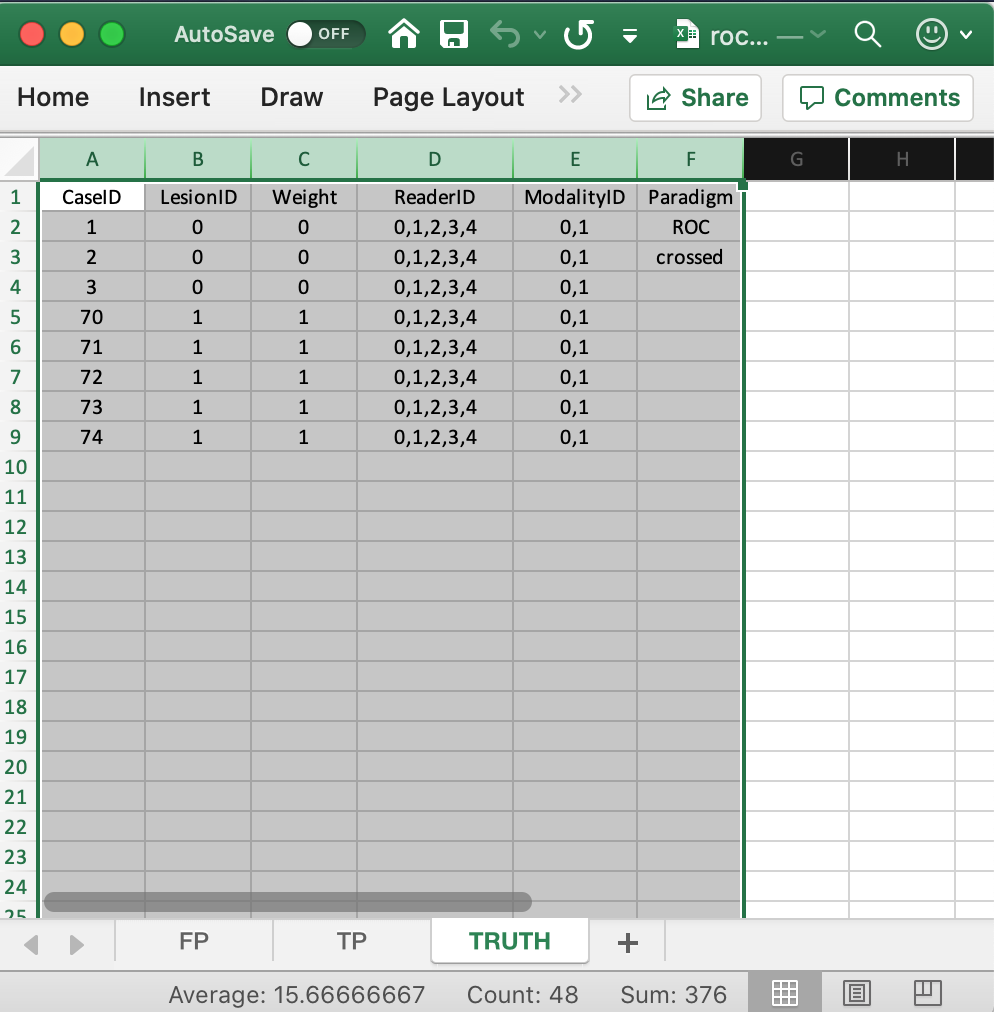
\includegraphics[width=0.5\linewidth,height=0.2\textheight]{images/rocCrTruth} 

}

\caption{Truth worksheet for file rocCr.xlsx}\label{fig:showRocCrTruthSheet}
\end{figure}

\hypertarget{the-structure-of-an-roc-dataset}{%
\section{The structure of an ROC dataset}\label{the-structure-of-an-roc-dataset}}

In the following code chunk the first statement retrieves the name of the data file, located in a hidden directory that one need not be concerned with. The second statement reads the file using the function \texttt{DfReadDataFile()} and saves it to object \texttt{x}. The third statement shows the structure of the dataset object \texttt{x}.

\begin{Shaded}
\begin{Highlighting}[]
\NormalTok{rocCr \textless{}{-}}\StringTok{ }\KeywordTok{system.file}\NormalTok{(}\StringTok{"extdata"}\NormalTok{, }\StringTok{"toyFiles/ROC/rocCr.xlsx"}\NormalTok{,}
                        \DataTypeTok{package =} \StringTok{"RJafroc"}\NormalTok{, }\DataTypeTok{mustWork =} \OtherTok{TRUE}\NormalTok{)}
\NormalTok{x \textless{}{-}}\StringTok{ }\KeywordTok{DfReadDataFile}\NormalTok{(rocCr, }\DataTypeTok{newExcelFileFormat =} \OtherTok{TRUE}\NormalTok{)}
\KeywordTok{str}\NormalTok{(x)}
\CommentTok{\#\textgreater{} List of 12}
\CommentTok{\#\textgreater{}  $ NL           : num [1:2, 1:5, 1:8, 1] 1 3 2 3 2 2 1 2 3 2 ...}
\CommentTok{\#\textgreater{}  $ LL           : num [1:2, 1:5, 1:5, 1] 5 5 5 5 5 5 5 5 5 5 ...}
\CommentTok{\#\textgreater{}  $ lesionVector : int [1:5] 1 1 1 1 1}
\CommentTok{\#\textgreater{}  $ lesionID     : num [1:5, 1] 1 1 1 1 1}
\CommentTok{\#\textgreater{}  $ lesionWeight : num [1:5, 1] 1 1 1 1 1}
\CommentTok{\#\textgreater{}  $ dataType     : chr "ROC"}
\CommentTok{\#\textgreater{}  $ modalityID   : Named chr [1:2] "0" "1"}
\CommentTok{\#\textgreater{}   ..{-} attr(*, "names")= chr [1:2] "0" "1"}
\CommentTok{\#\textgreater{}  $ readerID     : Named chr [1:5] "0" "1" "2" "3" ...}
\CommentTok{\#\textgreater{}   ..{-} attr(*, "names")= chr [1:5] "0" "1" "2" "3" ...}
\CommentTok{\#\textgreater{}  $ design       : chr "CROSSED"}
\CommentTok{\#\textgreater{}  $ normalCases  : int [1:3] 1 2 3}
\CommentTok{\#\textgreater{}  $ abnormalCases: int [1:5] 70 71 72 73 74}
\CommentTok{\#\textgreater{}  $ truthTableStr: num [1:2, 1:5, 1:8, 1:2] 1 1 1 1 1 1 1 1 1 1 ...}
\end{Highlighting}
\end{Shaded}

\begin{itemize}
\tightlist
\item
  In the above code chunk flag \texttt{newExcelFileFormat} is set to \texttt{TRUE} as otherwise columns D - F in the \texttt{Truth} worksheet are ignored and the dataset is assumed to be crossed, with \texttt{dataType} automatically determined from the contents of the FP and TP worksheets.
\item
  Flag \texttt{newExcelFileFormat\ =\ FALSE} is for compatibility with older JAFROC format Excel files, which did not have these columns in the \texttt{Truth} worksheet. Its usage is deprecated.
\item
  The dataset object \texttt{x} is a \texttt{list} variable with 12 members.
\item
  The \texttt{x\$NL} member, with dimension {[}2, 5, 8, 1{]}, contains the ratings of normal cases. The extra values in the third dimension, filled with \texttt{NAs}, are needed for compatibility with FROC datasets, as unlike ROC, false positives are possible on diseased cases.
\item
  The \texttt{x\$LL}, with dimension {[}2, 5, 5, 1{]}, contains the ratings of abnormal cases.
\item
  The \texttt{x\$lesionVector} member is a vector with 5 ones representing the 5 diseased cases in the dataset.
\item
  The \texttt{x\$lesionID} member is an array with 5 ones.
\item
  The \texttt{x\$lesionWeight} member is an array with 5 ones.
\item
  The \texttt{lesionVector}, \texttt{lesionID} and \texttt{lesionWeight} members are not used for ROC datasets. They are there for compatibility with FROC datasets.
\item
  The \texttt{dataType} member indicates that this is an \texttt{ROC} dataset.
\item
  The \texttt{x\$modalityID} member is a vector with two elements \texttt{"0"} and \texttt{"1"}, naming the two modalities.
\item
  The \texttt{x\$readerID} member is a vector with five elements \texttt{"0"}, \texttt{"1"}, \texttt{"2"}, \texttt{"3"} and \texttt{"4"}, naming the five readers.
\item
  The \texttt{x\$design} member is CROSSED; specifies the dataset design, which is ``CROSSED''.
\item
  The \texttt{x\$normalCases} member lists the integer names of the normal cases, 1, 2, 3.
\item
  The \texttt{x\$abnormalCases} member lists the integer names of the abnormal cases, 70, 71, 72, 73, 74.
\item
  The \texttt{x\$truthTableStr} member quantifies the structure of the dataset, as explained in \textbf{Chapter 00 Vignette \#3-\#5}.
\end{itemize}

\hypertarget{the-false-positive-fp-ratings}{%
\section{The false positive (FP) ratings}\label{the-false-positive-fp-ratings}}

These are found in the \texttt{FP} or \texttt{NL} worksheet, see below.

\begin{figure}

{\centering 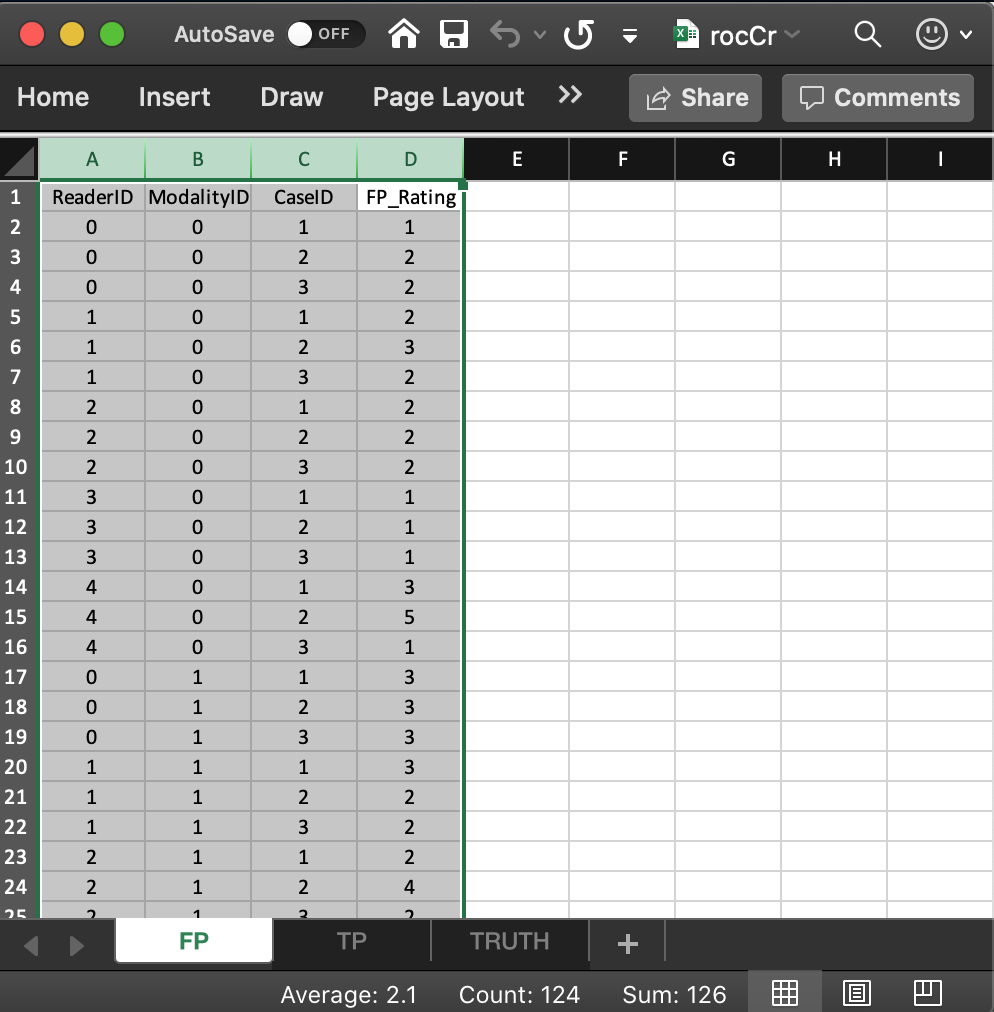
\includegraphics[width=0.5\linewidth,height=0.2\textheight]{images/rocCrFp} 

}

\caption{FP worksheet for file rocCr.xlsx}\label{fig:showRocCrFpSheet}
\end{figure}

\begin{itemize}
\tightlist
\item
  It consists of 4 columns, each of length 30 (= \# of modalities times number of readers times number of non-diseased cases).
\item
  \texttt{ReaderID}: the reader labels: \texttt{0}, \texttt{1}, \texttt{2}, \texttt{3} and \texttt{4}. Each reader label occurs 6 times (= \# of modalities times number of non-diseased cases).
\item
  \texttt{ModalityID}: the modality or treatment labels: \texttt{0} and \texttt{1}. Each label occurs 15 times (= \# of readers times number of non-diseased cases).
\item
  \texttt{CaseID}: the case labels for non-diseased cases: \texttt{1}, \texttt{2} and \texttt{3}. Each label occurs 10 times (= \# of modalities times \# of readers).
\item
  The label of a diseased case cannot occur in the FP worksheet. If it does the software generates an error.
\item
  \texttt{FP\_Rating}: the floating point ratings of non-diseased cases. Each row of this worksheet contains a rating corresponding to the values of \texttt{ReaderID}, \texttt{ModalityID} and \texttt{CaseID} for that row.
\end{itemize}

\hypertarget{the-true-positive-tp-ratings}{%
\section{The true positive (TP) ratings}\label{the-true-positive-tp-ratings}}

These are found in the \texttt{TP} or \texttt{LL} worksheet, see below.

\begin{figure}

{\centering 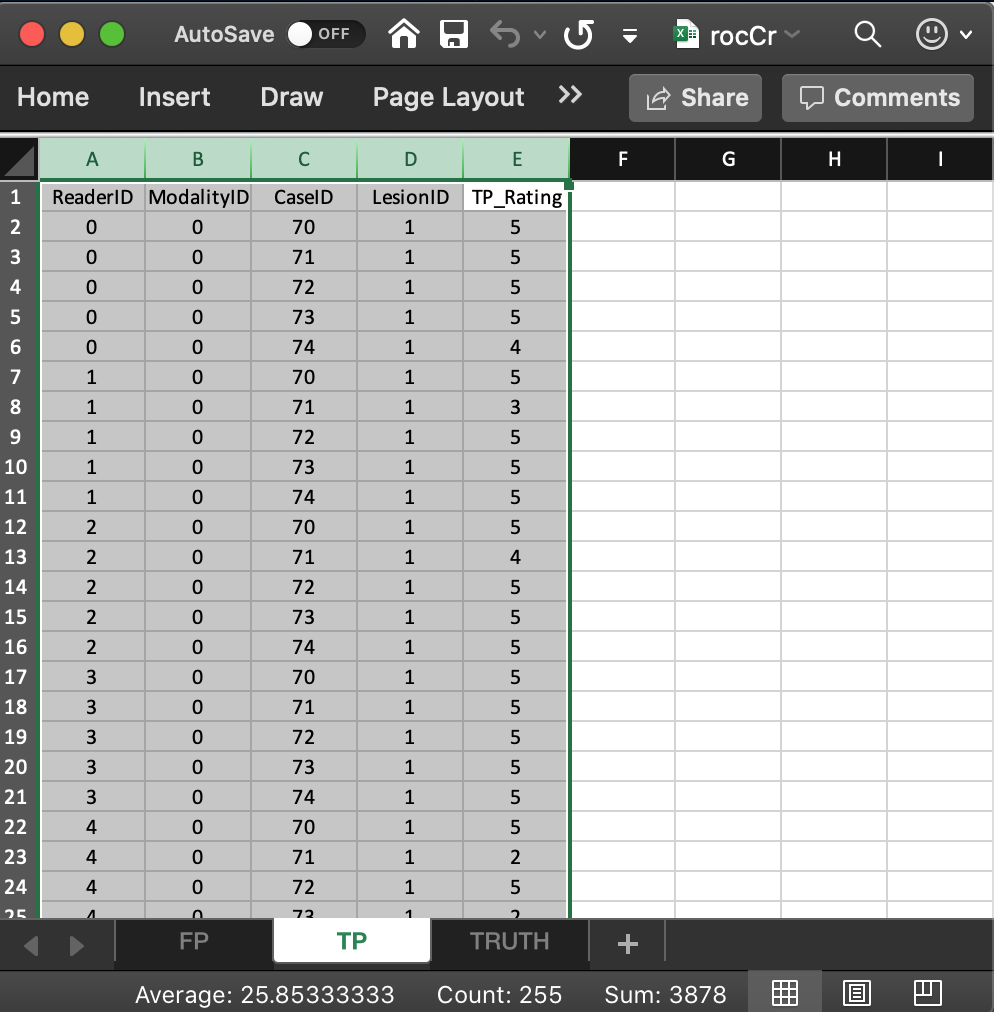
\includegraphics[width=0.5\linewidth,height=0.2\textheight]{images/rocCrTp} 

}

\caption{TP worksheet for file rocCr.xlsx}\label{fig:showRocCrTpSheet}
\end{figure}

\begin{itemize}
\tightlist
\item
  It consists of 5 columns, each of length 50 (= \# of modalities times number of readers times number of diseased cases).
\item
  \texttt{ReaderID}: the reader labels: \texttt{0}, \texttt{1}, \texttt{2}, \texttt{3} and \texttt{4}. Each reader label occurs 10 times (= \# of modalities times number of diseased cases).
\item
  \texttt{ModalityID}: the modality or treatment labels: \texttt{0} and \texttt{1}. Each label occurs 25 times (= \# of readers times number of diseased cases).
\item
  \texttt{LesionID}: For an ROC dataset this column contains fifty 1's (each diseased case has one lesion).
\item
  \texttt{CaseID}: the case labels for non-diseased cases: \texttt{70}, \texttt{71}, \texttt{72}, \texttt{73} and \texttt{74}. Each label occurs 10 times (= \# of modalities times \# of readers). The label of a non-diseased case cannot occur in the TP worksheet.
\item
  \texttt{TP\_Rating}: the floating point ratings of diseased cases. Each row of this worksheet contains a rating corresponding to the values of \texttt{ReaderID}, \texttt{ModalityID}, \texttt{LesionID} and \texttt{CaseID} for that row.
\end{itemize}

\hypertarget{correspondence-between-nl-member-of-dataset-and-the-fp-worksheet}{%
\section{\texorpdfstring{Correspondence between \texttt{NL} member of dataset and the \texttt{FP} worksheet}{Correspondence between NL member of dataset and the FP worksheet}}\label{correspondence-between-nl-member-of-dataset-and-the-fp-worksheet}}

\begin{itemize}
\tightlist
\item
  The list member \texttt{x\$NL} is an array with \texttt{dim\ =\ c(2,5,8,1)}.

  \begin{itemize}
  \tightlist
  \item
    The first dimension (2) comes from the number of modalities.
  \item
    The second dimension (5) comes from the number of readers.
  \item
    The third dimension (8) comes from the \textbf{total} number of cases.
  \item
    The fourth dimension is alway 1 for an ROC dataset.
  \end{itemize}
\item
  The value of \texttt{x\$NL{[}1,5,2,1{]}}, i.e., 5, corresponds to row 15 of the FP table, i.e., to \texttt{ModalityID} = 0, \texttt{ReaderID} = 4 and \texttt{CaseID} = 2.
\item
  The value of \texttt{x\$NL{[}2,3,2,1{]}}, i.e., 4, corresponds to row 24 of the FP table, i.e., to \texttt{ModalityID} 1, \texttt{ReaderID} 2 and \texttt{CaseID} 2.
\item
  All values for case index \textgreater{} 3 are \texttt{-Inf}. For example the value of \texttt{x\$NL{[}2,3,4,1{]}} is \texttt{-Inf}. This is because there are only 3 non-diseased cases. The extra length is needed for compatibility with FROC datasets.
\end{itemize}

\hypertarget{correspondence-between-ll-member-of-dataset-and-the-tp-worksheet}{%
\section{\texorpdfstring{Correspondence between \texttt{LL} member of dataset and the \texttt{TP} worksheet}{Correspondence between LL member of dataset and the TP worksheet}}\label{correspondence-between-ll-member-of-dataset-and-the-tp-worksheet}}

\begin{itemize}
\tightlist
\item
  The list member \texttt{x\$LL} is an array with \texttt{dim\ =\ c(2,5,5,1)}.

  \begin{itemize}
  \tightlist
  \item
    The first dimension (2) comes from the number of modalities.
  \item
    The second dimension (5) comes from the number of readers.
  \item
    The third dimension (5) comes from the number of diseased cases.
  \item
    The fourth dimension is alway 1 for an ROC dataset.
  \end{itemize}
\item
  The value of \texttt{x\$LL{[}1,1,5,1{]}}, i.e., 4, corresponds to row 6 of the TP table, i.e., to \texttt{ModalityID} = 0, \texttt{ReaderID} = 0 and \texttt{CaseID} = 74.
\item
  The value of \texttt{x\$LL{[}1,2,2,1{]}}, i.e., 3, corresponds to row 8 of the TP table, i.e., to \texttt{ModalityID} = 0, \texttt{ReaderID} = 1 and \texttt{CaseID} = 71.
\item
  There are no -Inf values in \texttt{x\$LL}: \texttt{any(x\$LL\ ==\ -Inf)} = FALSE.
\end{itemize}

\hypertarget{correspondence-using-the-which-function}{%
\section{\texorpdfstring{Correspondence using the \texttt{which} function}{Correspondence using the which function}}\label{correspondence-using-the-which-function}}

\begin{itemize}
\tightlist
\item
  Converting from \textbf{names} to \textbf{subscripts} (indicating position in an array) can be confusing.
\item
  The following example uses the \texttt{which} function to help out.
\item
  The first line says that the \texttt{abnormalCase} named 70 corresponds to subscript 1 in the LL array case dimension.
\item
  The second line prints the NL rating for \texttt{modalityID} = 0, \texttt{readerID} = 1 and \texttt{normalCases} = 1.
\item
  The third line prints the LL rating for \texttt{modalityID} = 0, \texttt{readerID} = 1 and \texttt{abnormalCases} = 70.
\item
  The last line shows what happens if one enters an invalid value for name; the result is a \texttt{numeric(0)}.
\item
  Note that in each of these examples, the last dimension is 1 because we are dealing with an ROC dataset.
\item
  The reader is encouraged to examine the correspondence between the NL and LL ratings and the Excel file using this method.
\end{itemize}

\begin{Shaded}
\begin{Highlighting}[]
\KeywordTok{which}\NormalTok{(x}\OperatorTok{$}\NormalTok{abnormalCases }\OperatorTok{==}\StringTok{ }\DecValTok{70}\NormalTok{)}
\CommentTok{\#\textgreater{} [1] 1}
\NormalTok{x}\OperatorTok{$}\NormalTok{NL[}\KeywordTok{which}\NormalTok{(x}\OperatorTok{$}\NormalTok{modalityID }\OperatorTok{==}\StringTok{ "0"}\NormalTok{),}\KeywordTok{which}\NormalTok{(x}\OperatorTok{$}\NormalTok{readerID }\OperatorTok{==}\StringTok{ "1"}\NormalTok{),}\KeywordTok{which}\NormalTok{(x}\OperatorTok{$}\NormalTok{normalCases }\OperatorTok{==}\StringTok{ }\DecValTok{1}\NormalTok{),}\DecValTok{1}\NormalTok{]}
\CommentTok{\#\textgreater{} [1] 2}
\NormalTok{x}\OperatorTok{$}\NormalTok{LL[}\KeywordTok{which}\NormalTok{(x}\OperatorTok{$}\NormalTok{modalityID }\OperatorTok{==}\StringTok{ "0"}\NormalTok{),}\KeywordTok{which}\NormalTok{(x}\OperatorTok{$}\NormalTok{readerID }\OperatorTok{==}\StringTok{ "1"}\NormalTok{),}\KeywordTok{which}\NormalTok{(x}\OperatorTok{$}\NormalTok{abnormalCases }\OperatorTok{==}\StringTok{ }\DecValTok{70}\NormalTok{),}\DecValTok{1}\NormalTok{]}
\CommentTok{\#\textgreater{} [1] 5}
\NormalTok{x}\OperatorTok{$}\NormalTok{LL[}\KeywordTok{which}\NormalTok{(x}\OperatorTok{$}\NormalTok{modalityID }\OperatorTok{==}\StringTok{ "a"}\NormalTok{),}\KeywordTok{which}\NormalTok{(x}\OperatorTok{$}\NormalTok{readerID }\OperatorTok{==}\StringTok{ "1"}\NormalTok{),}\KeywordTok{which}\NormalTok{(x}\OperatorTok{$}\NormalTok{abnormalCases }\OperatorTok{==}\StringTok{ }\DecValTok{70}\NormalTok{),}\DecValTok{1}\NormalTok{]}
\CommentTok{\#\textgreater{} numeric(0)}
\end{Highlighting}
\end{Shaded}

\hypertarget{references-1}{%
\section{References}\label{references-1}}

  \bibliography{packages.bib,myRefs.bib}

\end{document}
